% LaTeX mintafájl szakdolgozat és diplomamunkáknak az
% SZTE Informatikai Tanszékcsoportja által megkövetelt
% formai követelményeinek megvalósításához
% Modosítva: 2011.04.28 Nemeth L. Zoltan
% A fájl használatához szükséges a magyar.ldf 2005/05/12 v1.5-ös vagy későbbi verziója
% ez letölthető a http://www.math.bme.hu/latex/ weblapról, a magyar nyelvű szedéshez
% Hasznos információk, linekek, LaTeX leírások a www.latex.lap.hu weboldalon vannak.
%

\documentclass[12pt]{report}

%Magyar nyelvi támogatás (Babel 3.7 vagy későbbi kell!)
\def\magyarOptions{defaults=hu-min}
\usepackage[magyar]{babel}

%Az ékezetes betűk használatához:
\usepackage{t1enc}% ékezetes szavak automatikus elválasztásához
\usepackage[utf8]{inputenc}% ékezetes szavak beviteléhez

% A formai kovetelmenyekben megkövetelt Times betűtípus használata:
\usepackage{times}

%Az AMS csomagjai
\usepackage{amsmath}
\usepackage{amssymb}
\usepackage{amsthm}

%A fejléc láblécek kialakításához:
\usepackage{fancyhdr}

%Természetesen további csomagok is használhatók,
%például ábrák beillesztéséhez a graphix és a psfrag,
%ha nincs rájuk szükség természetesen kihagyhatók.
\usepackage{graphicx}
\usepackage{psfrag}

\usepackage{setspace}

\usepackage{hyperref}
\hypersetup{
    colorlinks,
    citecolor=black,
    filecolor=black,
    linkcolor=black,
    urlcolor=black
}

\usepackage{cite}

%\usepackage{enumitem}
\usepackage{enumerate}

% Színek
\usepackage{color}
\definecolor{myCommentColorGreen}{RGB}{0,128,0}
\definecolor{myLineNumberGray}{RGB}{128,128,128}

% Forráskódhoz
\usepackage{listings}
\lstset{ %
    %backgroundcolor=\color{white},   % choose the background color; you must add  \usepackage{color} or \usepackage{xcolor}
    basicstyle=\footnotesize,         % the size of the fonts that are used for    the code
    %breakatwhitespace=false,         % sets if automatic breaks should only      happen at whitespace
    breaklines=true,                  % sets automatic line breaking          captionpos=b,                    % sets the caption-position to          bottom
    commentstyle=\color{myCommentColorGreen},    % comment style
    %deletekeywords={...},            % if you want to delete keywords              from the given language
    %escapeinside={\%*}{*)},          % if you want to add LaTeX                within your code
    %extendedchars=true,              % lets you use non-ASCII                  characters; for 8-bits encodings only, does not work with                  UTF-8
    frame=leftline,                   % adds a frame around the                    code
    %keepspaces=true,                 % keeps spaces in text,                      useful for keeping indentation of code (possibly needs                      columns=flexible)
    inputpath=../../../code/gepard,
    keywordstyle=\color{blue},        % keyword style
    language=C++,                     % the language of                          the code
    %morekeywords={*,...},            % if you want to                            add more keywords to the set
    numberfirstline=true,
    numbers=left,                     % where to put                              the line-numbers; possible values are (none, left, right)
    numbersep=10pt,                   % how far theline-numbers are from the code
    numberstyle=\tiny\color{myLineNumberGray}, % the stylethat is used for the line-numbers
    %name=\thelstnumber,              %
    %rulecolor=\color{black},         % if notset, the frame-color may be changed online-breaks within not-black text (e.g.comments (green here))
    %showspaces=false,                % showspaces everywhere adding particularunderscores; it overrides'showstringspaces'
    %showstringspaces=false,          % underline spaces within strings only
    %showtabs=false,                  % show tabs within strings addingparticular underscores
    %stepnumber=2,                    % the step between two line-numbers.If it's 1, each line will benumbered
    %stringstyle=\color{mymauve},     % string literal style
    tabsize=4,                        % sets default tabsize to 2    spaces
    %title=\lstname                   % show the filename of     files included with     \lstinputlisting; also try     caption instead of title
}

% Kép mellett folyó íráshoz
\usepackage{wrapfig}

%Tételszerű környezetek definiálhatók, ezek most fejezetenként együtt számozódnak, pl.
\newtheorem{tét}{Tétel}[chapter]
\newtheorem{defi}[tét]{Definíció}
\newtheorem{lemma}[tét]{Lemma}
\newtheorem{áll}[tét]{Állítás}
\newtheorem{köv}[tét]{Következmény}

%Ha a megjegyzések és a példak szövegét nem akarjuk dőlten szedni, akkor
%az alábbi parancs után kell őket definiální:
\theoremstyle{definition}
\newtheorem{megj}[tét]{Megjegyzés}
\newtheorem{pld}[tét]{Példa}

%%% Saját parancsok
% Az angol kifejezések kiemelése
\newcommand{\inenglish}[1]{\textsl{#1}}
\newcommand{\inenglishfn}[1]{\footnotesize{\inenglish{#1}}}

%\hyphenation{sza-bály el-kü-lö-ní-tett}

%Margók:
\hoffset -1in
\voffset -1in
\oddsidemargin 35mm
\textwidth 150mm
\topmargin 15mm
\headheight 10mm
\headsep 5mm
\textheight 237mm

\begin{document}


%%%%%%%%%%%%%%%%%%%%%%%%%%%%%%%%%%%%%%%%%%%%%%%%%%%%%%%%%%%%%%%%%%%%%%
%%   Címlap                                                         %%
%%%%%%%%%%%%%%%%%%%%%%%%%%%%%%%%%%%%%%%%%%%%%%%%%%%%%%%%%%%%%%%%%%%%%%

    %A FEJEZETEK KEZDŐOLDALAINAK FEJ ÉS LÁBLÉCE:
    %a plain oldalstílust kell átdefiniálni, hogy ott ne legyen fejléc:
    \fancypagestyle{plain}{%
    %ez mindent töröl:
    \fancyhf{}
    % a láblécbe jobboldalra kerüljön az oldalszám:
    \fancyfoot[R]{\thepage}
    %elválasztó vonal sem kell:
    \renewcommand{\headrulewidth}{0pt}
    }

    %A TÖBBI OLDAL FEJ ÉS LÁBLÉCE:
    \pagestyle{fancy}
    \fancyhf{}
    \fancyhead[L]{OpenGL-ES 2.0 alapú Path API}
    \fancyfoot[R]{\thepage}


    %A címoldalra se fej- se lábléc nem kell:
    \thispagestyle{empty}

    \begin{center}
    \vspace*{1cm}
    {\Large\bf Szegedi Tudományegyetem}

    \vspace{0.5cm}

    {\Large\bf Informatikai Tanszékcsoport}

    \vspace*{3.8cm}

    % Tíz sorral fentebb is át kell írni!!!
    {\LARGE\bf OpenGL-ES 2.0 alapú Path API}


    \vspace*{3.6cm}

    {\Large Diplomamunka}
    % vagy {\Large Szakdolgozat}

    \vspace*{4cm}

    %Értelemszerűen megváltoztatandó:
    {\large
    \begin{tabular}{c@{\hspace{4cm}}c}
    \emph{Készítette:}     &\emph{Témavezető:}\\
    \bf{Ledán Szilárd}  &\bf{Dr. Kiss Ákos}\\
    informatika szakos     & adjunktus\\
    hallgató &
    \end{tabular}
    }

    \vspace*{2.3cm}

    {\Large
    Szeged
    \\
    \vspace{2mm}
    2016
    }
    \end{center}


    % 1.5-ös sorköz:
    % ezt javasolják:  \linespread{1.25}
    % és ez bevált, de ehhez kellett a \usepackage{setspace} csomag betöltése.
    \onehalfspacing


%%%%%%%%%%%%%%%%%%%%%%%%%%%%%%%%%%%%%%%%%%%%%%%%%%%%%%%%%%%%%%%%%%%%%%
%%   Tartalomjegyzék                                                %%
%%%%%%%%%%%%%%%%%%%%%%%%%%%%%%%%%%%%%%%%%%%%%%%%%%%%%%%%%%%%%%%%%%%%%%

    \tableofcontents


%%%%%%%%%%%%%%%%%%%%%%%%%%%%%%%%%%%%%%%%%%%%%%%%%%%%%%%%%%%%%%%%%%%%%%
%%   Feladatkiírás                                                  %%
%%%%%%%%%%%%%%%%%%%%%%%%%%%%%%%%%%%%%%%%%%%%%%%%%%%%%%%%%%%%%%%%%%%%%%


    %A \chapter* parancs nem ad a fejezetnek sorszámot
    \chapter*{Feladatkiírás}
    %A tartalomjegyzékben mégis szerepeltetni kell, mint szakasz(section) szerepeljen:
    \addcontentsline{toc}{section}{Feladatkiírás}

A témavezető által megfogalmazott feladatkiírás. Önálló oldalon szerepel.


%%%%%%%%%%%%%%%%%%%%%%%%%%%%%%%%%%%%%%%%%%%%%%%%%%%%%%%%%%%%%%%%%%%%%%
%%   Tartalmi összefoglaló                                          %%
%%%%%%%%%%%%%%%%%%%%%%%%%%%%%%%%%%%%%%%%%%%%%%%%%%%%%%%%%%%%%%%%%%%%%%

    \chapter*{Tartalmi összefoglaló}
    \addcontentsline{toc}{section}{Tartalmi összefoglaló}

%A tartalmi összefoglalónak tartalmaznia kell (rövid, legfeljebb egy oldalas, összefüggő megfogalmazásban)
%a következőket: a téma megnevezése, a megadott feladat megfogalmazása - a feladatkiíráshoz viszonyítva-,
%a megoldási mód, az alkalmazott eszközök, módszerek, az elért eredmények, kulcsszavak (4-6 darab).

%Az összefoglaló nyelvének meg kell egyeznie a dolgozat nyelvével. Ha a dolgozat idegen nyelven készül,
%magyar nyelvű tartalmi összefoglaló készítése is kötelező (külön lapon), melynek terjedelmét a TVSZ szabályozza.

    \subsubsection*{A téma megnevezése}

  A \emph{W3C} (World Wide Web Consortium) által \emph{Canvas 2D
Context} néven 2015-ben elfogadott ajánlás \emph{path} részének
megvalósítása \emph{OpenGL-ES 2.0} alapokon.

    \subsubsection*{A megadott feladat megfogalmazása}

  Az előbb említett \emph{Canvas} egy grafikus API~\footnote{Az
alkalmazásprogramozási felület/interfész (Application Programming
Interface) kifejezésre a továbbiakban mint \emph{API}
hivatkozunk.}.
  Ez az API több grafikus függvényt definiál (ld. később).
  Jelen dolgozat témája ezek közül az úgynevezett \emph{path} részének
leprogramozása~úgy, hogy a lehető legtöbb feladatot a grafikus
processzor (\textit{GPU}) lássa el.

    \subsubsection*{A megoldásmód}

  Több megoldás közül (ld. a Háttér részt) mi az alakzatok trapézokra
bontását választottuk. Hiszen minden trapéz felbontható további két
háromszögre, mely megkötésre a GLES2 grafikus renderelő~\footnote{Az
előállítás--megjelenítés (\emph{rendering}) kifejezésre a
továbbiakban \emph{renderelés}ként hívatkozunk.} API miatt van
szükség.

    \subsubsection*{Alkalmazott eszközök, módszerek}

  Az API \emph{c++11} programozási nyelven készült, használva a
következő eszközöket, technológiákat: \emph{gcc}, \emph{git},
\textit{OpenGL ES 2.0}, \emph{\LaTeX},

    \subsubsection*{Elért eredmények}

    \subsubsection*{Kulcsszavak}

grafika, path, canvas-2D-context, OpenGL-ES 2.0


%%%%%%%%%%%%%%%%%%%%%%%%%%%%%%%%%%%%%%%%%%%%%%%%%%%%%%%%%%%%%%%%%%%%%%
%%   Bevezetés                                                      %%
%%%%%%%%%%%%%%%%%%%%%%%%%%%%%%%%%%%%%%%%%%%%%%%%%%%%%%%%%%%%%%%%%%%%%%

    \chapter*{Bevezetés}
    \label{Bevezetés}
    \addcontentsline{toc}{section}{Bevezetés}

  A környezetünkben található számítástechnikai eszközök
legtöbbjének van grafikus kijelzője, és ezen eszközök mindegyike használ
valamilyen megjelenítő~\footnote{A számítógépes grafikában egy modell
megjelenítését végző folyamatot \emph{renderelés}nek (\inenglishfn{rendering}),
a renderelést végző programrészt pedig \emph{motor}nak (\inenglishfn{engine})
hívnak} (a továbbiakban renderelő) függvénykönyvtárat. Ilyen például a Skia, a
Cairo, az OpenGL, és ilyen tervezését tűzte ki célul a Gepard Graphics is. A
\emph{Gepard} a tervek szerint egy \emph{C++11}-es nyelven írt, és több
(OpenGL, \mbox{OpenGL-ES 2.0\cite{Munshi:2008:OEP:1481069}} és Vulkan) grafikus
renderelő motort támogató függvénykönyvtár lesz.

  A tervek szerint idővel a Gepard több interfésszel is rendelkezik.
Így alkot majd egy komplex grafikus alkalmazásprogramozási felületet
(\inenglish{Application Programming Interface}, a továbbiakban API). Az elsőnek
választott ilyen ismertebb interfész amit támogatni kíván az a \emph{W3C} által
készített \emph{Canvas 2D Context}~\cite{Cabanier:14:HCC} nevű ajánlás.

  A \emph{Canvas 2D Context} (a továbbiakban \emph{Canvas}) ajánlás
2015-ös kiadása több elkülönített részből állítja össze az API-t. Ezen részek
egyike az úgynevezett \emph{path}. Az említett 2015-ös ajánlás az 5., 8. és 11.
fejezetekben részletezi a pathszal szembeni elvárásokat. A path maga a
definiált grafikus alakzatokhoz képest bonyolultabbak leírását biztosító
eszköz. A Háttér (\ref{Háttér}.) fejezetben részletesebben kifejtjük a patht
építő eszköz lehetőségeit és szabályait. Itt most csak annyiban kell kitérjünk
rá, hogy alapvetően két nagyobb részből áll ez is. A \emph{körvonalból}
(\inenglish{stroke}) és a \emph{kitöltésből} (\inenglish{fill}).

  Jelen dolgozat a kitöltést megvalósító részt kívánja bemutatni.
Azt, hogy milyen szabályoknak kellett megfelelni, milyen lehetőségeket
biztosított a választott OpenGL-ES 2.0 (a továbbiakban GLES2) szabvány, és azt,
hogy hogyan alkot köztes réteget ezek között a Gepard path kitöltését biztosító
része.

  Első körben nem volt cél a ,,leggyorsabban futó'' és ,,legkisebb
méretű'' patht kitöltő renderelő API elkészítése. Célunk egy út megtalálása és
e mentén egy olyan eszköz megalkotása volt, amely képes a választott ajánlás
(Canvas) elvárásait teljesíteni. Valamint ezáltal megismerhetünk bizonyos
módszereket és technológiákat.


%%%%%%%%%%%%%%%%%%%%%%%%%%%%%%%%%%%%%%%%%%%%%%%%%%%%%%%%%%%%%%%%%%%%%%
%%   Háttér                                                         %%
%%%%%%%%%%%%%%%%%%%%%%%%%%%%%%%%%%%%%%%%%%%%%%%%%%%%%%%%%%%%%%%%%%%%%%

    \chapter{Háttér}
    \label{Háttér}

  Ebben a fejezetben tárgyaljuk azokat a technológiákat és kihívásokat,
amelyek keretet szabtak a feladatunknak. Beszélni kell magáról a Canvas
ajánlásról, a GLES2 szabvány nyújtotta lehetőségekről, azokról a matematikai
módszerekről, amelyek biztosítják számunkra, hogy tetszőlegesen bonyolult --
szerencsénkre zárt -- alakzatok kitöltését helyesen elvégezhessük. Össze
kellett kapcsolni a választott GLES2 szabta megkötést~\footnote { Az OpenGL 2.0
legfeljebb háromszögeket rajzol. } a Canvas Path API elvárásaival~\footnote {
Elvárás a tetszőleges számú körcikk, szakasz és Bézier-görbe alkotta -- akár
önmetsző -- alakzat mérethelyes megjelenítése. }. Ehhez több lépésbeli
megközelítést (\inenglish{approximation}) alkalmaztunk. Ezekről a lépésekről is
érdemes lesz beszélni.

    \section[A Canvas ajánlás]{A W3C Canvas 2D Context ajánlása}
    \label{A Canvas ajánlás}
%    \addcontentsline{toc}{subsection}{az ajánlás}

  A Canvas API egy közel tíz éves, kiforrott technológia~\footnote {A W3C első
HTML5 szabvány-vázlata:\\ \footnotesize{
\url{https://www.w3.org/TR/2008/WD-html5-20080122/\#the-2d}} }. Az ajánlás leír
egy felbontásfüggő rajzolóvásznat, amelyet jellemzően \emph{canvas}nek
neveznek. A canvas definició szerint nem más mint egy adott \emph{szélesség}gel
és \emph{hosszúság}gal meghatározott terület, ahova különböző alakzatokat,
képeket, szövegeket és egyéb nem dinamikus grafikai elemeket rakhatunk fel. Az
elemeket a canvashez tartozó \emph{context} gyűjti, és bizonyos parancsok
(pl.~\emph{fill}) esetén az addig összegyűjtötteket kirajzolja a megadott
sorrendben. Végül mindig egy \emph{kép} (\inenglish{image}) vagy még
pontosabban egy \emph{bit-térkép} (\inenglish{bitmap}) készül.

  Az ajánláson belül definiált Path API rész amúgy egy régebbi, elterjedt
alakzatszerkesztő eljáráson alapul. Az eljárás lényege, hogy bizonyos alap
eszközökkel definiálunk egy bonyolultabb formát. Ezt a folyamatot hívjuk
alakzat építésnek (\inenglish{path building}).

  Nézzük meg, milyen eszközöket biztosít a Path API.


A path építés
különböző elemek segítségével történik. Két fő részre bontható. Az első rész
tulajdonképpen nem is az építésre, mint inkább a definiálásra és a rajzolásra
vonatkozik. Míg a második rész tartalmazza a path építéséhet szükséges
parancsokat, elemeket. Ezek a parancsok vagy elemek a következők:

\begin{enumerate}[I.]
  \item Rajzoló parancsok:
    \begin{enumerate}
      \item \emph{beginPath}: egy állapot egyszerre csak egy
      \emph{path}t definiálhat. Ezzel a paranccsal kezdhetünk egy új
      patht építeni. Fontos azonban, hogy nem kötelező ezzel
      kezdeni, de az előtte épített részt viszont eldobja.
      Parancsforma:\newline
        \texttt{beginPath();}
      \item \emph{fill}: az addig felépített path-t
      \emph{kitöltéssel}, azaz a path által határolt belső részt
      a vászonra kirajzolja. Parancsforma:\newline
        \texttt{fill();}
      \item \emph{stroke}: az addig felépített path-t
      \emph{körvonallal}, azaz a path mentén a megfelelő
      vastagsággal a vászonra kirajzolja. Parancsforma:\newline
        \texttt{stroke();}
    \end{enumerate}
  \item Építő elemek, parancsok:
    \begin{enumerate}
      \item \emph{closePath}: egy megkezdett alakzatot bezár, azaz
      a legutolsó \emph{moveTo} elem koordinátáihoz húz egy
      egyenest egy \emph{lineTo} elem segítségével. Definíció
      szerint minden alakzat zárt, ezért ha még le nem zárt
      alakzatot próbálunk meg rajzolni, vagy egy \emph{moveTo}
      elemmel máshova ugranánk, akkor előtte ilyen parancs
      hívódik, hogy az bezáruljon.
      Parancsforma:\newline
        \texttt{closePath();}
      \item \emph{moveTo}: ha rajzoláskor egy képzeletbeli toll
      útjának tekintenénk az elemeket, akkor ez az elem a toll
      felemelése és adott pontba lehelyezése lenne. Innen kezdődik
      egy (zárt) alakzat rajzolása. Parancsforma:\newline
        \texttt{moveTo(x, y);}
      \item \emph{lineTo}: az előző pontból húz egy egyenest az
      argumentumban megadott koordinátába. Parancsforma:\newline
        \texttt{lineTo(x, y);}
      \item \emph{quadraticCurveTo}: az előző pontból az
      argumentumban megadott kontrollpont és végpont szerint húz
      egy másodrendű Bézier-görbét. Parancsforma:\newline
        \texttt{quadraticCurveTo(cpx, cpy, x, y);}
      \item \emph{bezierCurveTo}: az előző pontból az
      argumentumban megadott kontrollpontok és végpont szerint húz
      egy harmadrendű Bézier-görbét. Parancsforma:\newline
        \texttt{bezierCurveTo(cp1x, cp1y, cp2x, cp2y, x, y);}
      \item \emph{arcTo}: az előző pontból, akár egy
      \emph{lineTo} elem közbeékelésével a két kontrollpontnak
      és a sugárnak megfelelően egy körívet definiál úgy,
      hogy az a második pontban végződjék. Parancsforma:\newline
        \texttt{arcTo(x1, y1, x2, y2, radius);}
      \item \emph{rect}: egy külön zárt részalakzatot,
      méghozzá egy téglalapot definiál az argumentumoknak
      megfelelően. Ha nem volt bezárva az előző alakzat, akkor
      bezárja, illetve a téglalap kezdőpontjához állítja a
      végpontot (azaz innen folytathatjuk egy új részalakzat
      építését). Parancsforma:\newline
        \texttt{rect(x, y, w, h);}
      \item \emph{arc}: az argumentumoknak megfelelően egy
      körívet húz. Ha nem volt előző pont, akkor a
      középpontot tekinti annak, és a kezdő szög által
      definiált pontba egy \emph{lineTo} elemet iktat.
      Parancsforma:\newline
        \texttt{arc(x, y, radius, startAngle, endAngle, counterclockwise = false);}
    \end{enumerate}
\end{enumerate}

\Aref{dataflow-canvas-API-diagram}. ábrán láthatók az építő és rajzoló
elemek. Illetve feltüntettük még az ajánlásban nem szereplő
\emph{setFillColor} parancsot is. Ezzel a paranccsal adhatjuk meg a
contexthez tartozó aktuális kitöltő színt. Ez a parancs nem része
az ajánlásnak. Ott egy \emph{CSS DOM} elemmel állíthatjuk be ezt
az értéket. Az általunk tervezett API azonban csak a Canvas 2D
Contextre koncentrál, így a CSS elemeket nem kívánjuk támogatni.
    \begin{wrapfigure}{l}{0.5\textwidth}
    \begin{center}
      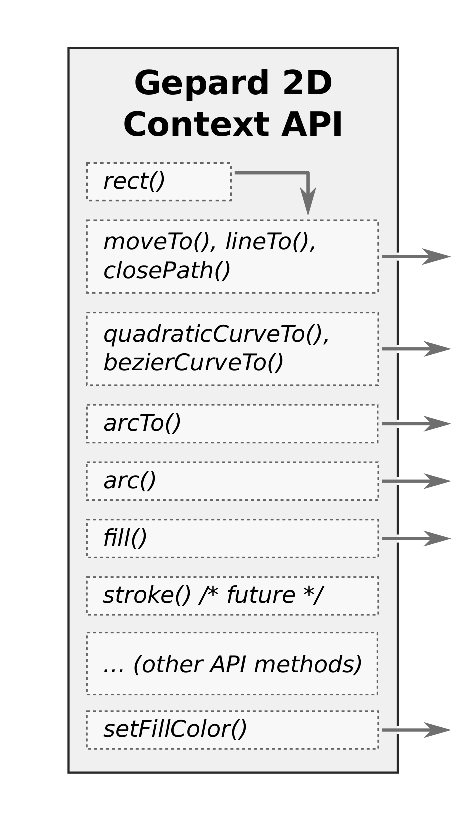
\includegraphics[scale=0.6]{img/dataflow_canvas_api_eps}
    \end{center}
      \caption{\label{dataflow-canvas-API-diagram}
      A Gepard Context 2D API}
    \end{wrapfigure}
Illetve nincs az ábrán a \emph{beginPath} parancs. Végül is az
jelen esetben nem több mint egy törlés és újrakezdés.

  Az ábrán a kimenő nyilak a Gepard belső APIjának a hívásait
jelölik. A \emph{rect} függvény esetében ez nem igényel többet
mint egy megfelelő \emph{moveTo}, három \emph{lineTo} és egy
\emph{closePath} hívást. Azaz visszavezetjük a Canvas 2D már
megvalósított függvényeire.

  Érdemes még néhány szót ejteni a \emph{stroke} hívásról is. Ez
a rész a jelen dolgozatnak nem témája. Viszont a jövőben ennek e
résznek a megvalósításakor -- legalábbis első körben -- úgy fogunk
eljárni, hogy visszavezetjük a strokeot a fillre. Lévén, hogy adott
szélességű stroke által lefedett területet felfoghatjuk úgy is mint egy
kitöltéssel rajzolt bonyolultabb alakzatot. Így a strokenak is a fill
lesz a lelke.

    \section[GLES2 API]{Az OpenGL-ES 2.0 API}
    \label{GLES2 API}

  Az OpenGL-ES azaz az OpenGL Embeded System 2.0-ás verziója a
Khronos Group által felügyelt grafikus meghajtó szabvány.

    \section[Matematikai háttér]{Matematikai háttér}
    \label{Matematikai háttér}

  TODO: Matematikai háttér bevezetője

    \subsection{Seprő-egyenesek}
    \label{Seprő-egyenesek}

  TODO: néhány szó az általános adott külső pontból húzott
félegyenesek által

    \subsection{Bézier-görbe és a de Casteljau felbontás}
    \label{Bézier-görbe és a de Casteljau felbontás}

  A

\begin{equation}
%
\mathbf{B}(t)=\sum_{i=0}^{3} B_i(t) \mathbf{b}_i %\nonumber
%\]
\end{equation}

ahol $\mathbf{B}(t)=(x(t), y(t))$ a $t\in[0,1]$ paraméter által

    \subsection{Körívek közelítése Bézier-görbékkel}
    \label{}

%%%%%%%%%%%%%%%%%%%%%%%%%%%%%%%%%%%%%%%%%%%%%%%%%%%%%%%%%%%%%%%%%%%%%%
%%   Path API                                                       %%
%%%%%%%%%%%%%%%%%%%%%%%%%%%%%%%%%%%%%%%%%%%%%%%%%%%%%%%%%%%%%%%%%%%%%%

    \chapter{Belső Path API}

  A \emph{Gepard} tervezésekor fontos szempont volt, hogy ne csak az
GLES2 API-val működjön. Lehetőséget kell kínálni, hogy a jövőben
több grafikus meghajtó közül lehessen választani. Mint például
az OpenGL, a Vulkan, DirectX, esetleg egy referencia szoftveres
képalkotó (\inenglish{renderer}). Ezért a Gepard külső API-ján
belül terveztünk egy belső API-t, amely már a választott
rendererrel rajzol. A mi esetünkben ez a belső API-nak a Path
része. Ez rajzol GLES2-t használva. Ebben a részben kell elvégezni
azokat az átalakításokat, visszavezetéseket, amelyeket ugyanitt
háromszögek formájában kirajzolunk.

  Ebben a fejezetben fogjuk bemutatni ennek a belső Path API-nak a
felépítését és működését. Elsőnek áttekintve a
felépítését, majd részletezve az egyes megoldásokat és
visszavezetéseket, közelítéseket.

    \section[Felépítése]{Felépítése}
    \label{Felépítése}

    \begin{wrapfigure}{l}{0.5\textwidth}
    \begin{center}
      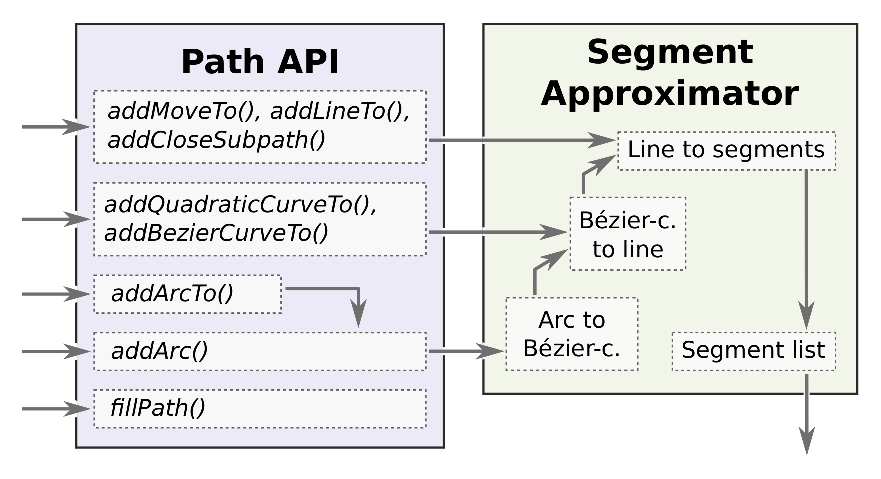
\includegraphics[scale=0.6]{img/dataflow_path_api_eps}
    \end{center}
      \caption{\label{dataflow-path-API-diagram} A belső Path API
      részei és a szakaszokra bontás fázisai}
    \end{wrapfigure}


    \begin{figure}[h]
    \centering
    \psfrag{t}[c][c]{$q_0$}
    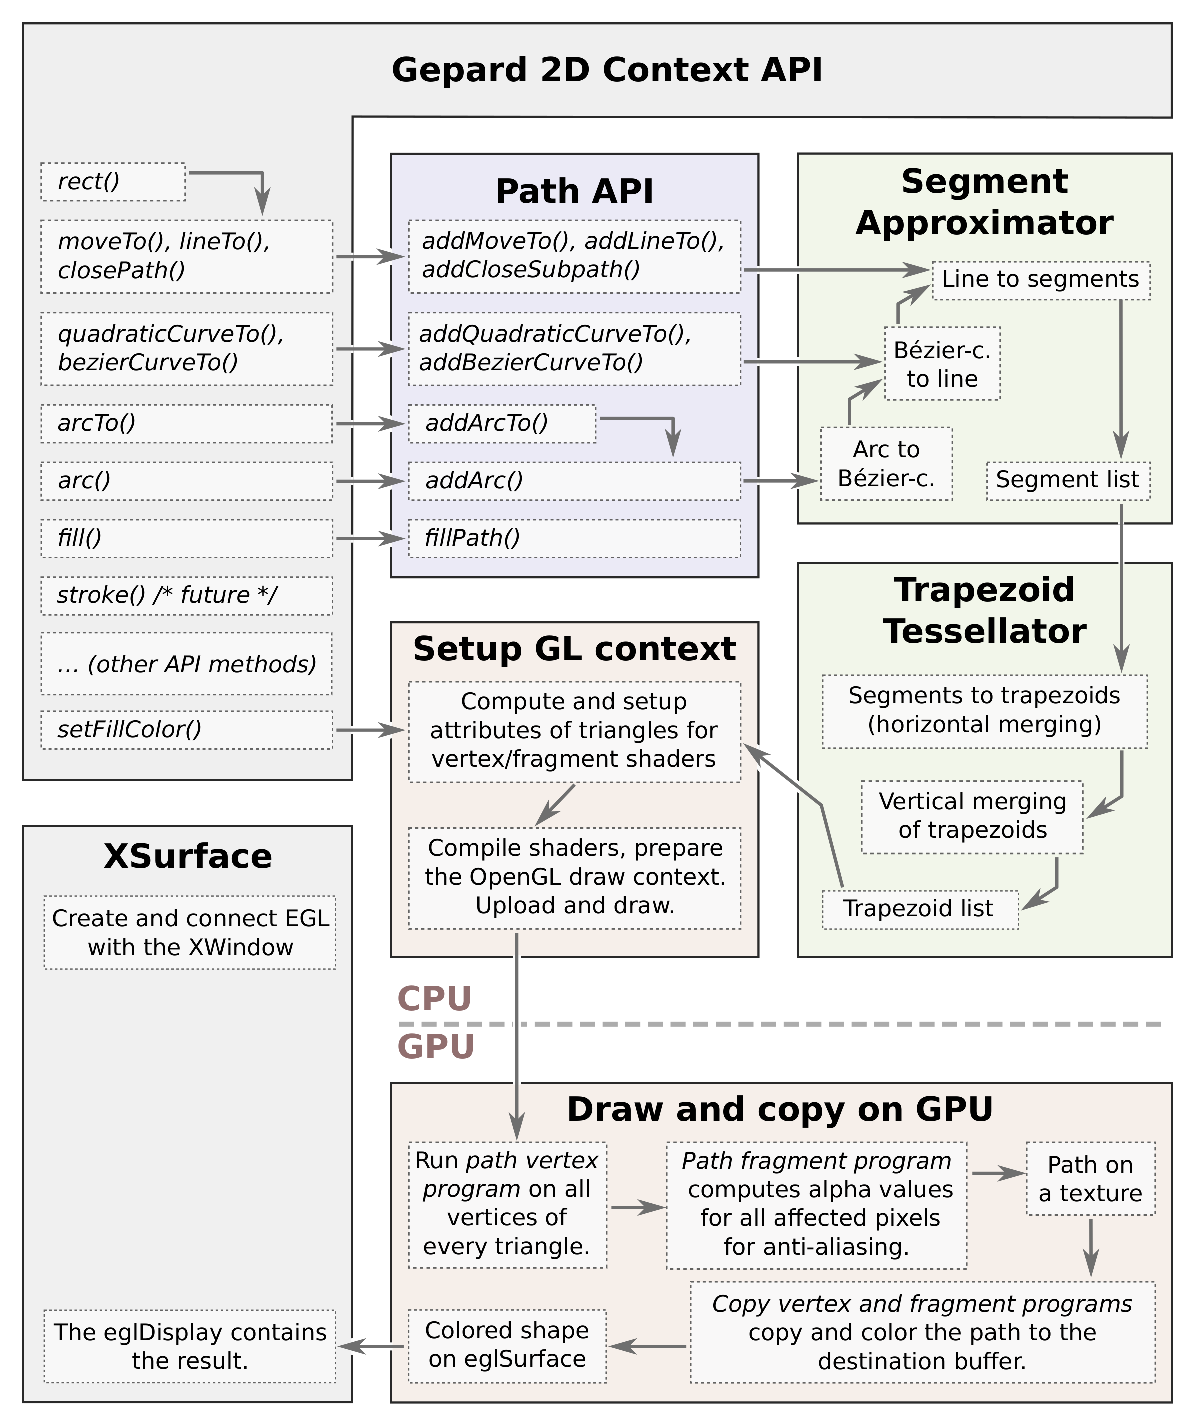
\includegraphics[scale=0.6]{img/dataflow_eps}
    \caption{\label{dataflow-diagram} A rajzolás folyamata}
    \end{figure}


%%%%%%%%%%%%%%%%%%%%%%%%%%%%%%%%%%%%%%%%%%%%%%%%%%%%%%%%%%%%%%%%%%%%%%
%%   Konklúzió                                                      %%
%%%%%%%%%%%%%%%%%%%%%%%%%%%%%%%%%%%%%%%%%%%%%%%%%%%%%%%%%%%%%%%%%%%%%%

    \chapter{Konklúzió}
    \addcontentsline{toc}{section}{Konklúzió}


%%%%%%%%%%%%%%%%%%%%%%%%%%%%%%%%%%%%%%%%%%%%%%%%%%%%%%%%%%%%%%%%%%%%%%
%%   Irodalomjegyzék                                                %%
%%%%%%%%%%%%%%%%%%%%%%%%%%%%%%%%%%%%%%%%%%%%%%%%%%%%%%%%%%%%%%%%%%%%%%

    \bibliography{bib/cites}{}
    \bibliographystyle{bib/huplain}

%%%%%%%%%%%%%%%%%%%%%%%%%%%%%%%%%%%%%%%%%%%%%%%%%%%%%%%%%%%%%%%%%%%%%%
%%   Nyilatkozat                                                    %%
%%%%%%%%%%%%%%%%%%%%%%%%%%%%%%%%%%%%%%%%%%%%%%%%%%%%%%%%%%%%%%%%%%%%%%

    \chapter*{Nyilatkozat}
    %Egy üres sort adunk a tartalomjegyzékhez:
    \addtocontents{toc}{\ }
    \addcontentsline{toc}{section}{Nyilatkozat}
    %\hspace{\parindent}

    % A nyilatkozat szövege más titkos és nem titkos dolgozatok esetében.
    % Csak az egyik típusú nyilatkozatnak kell a dolgozatban szerepelni
    % A pontok helyére az adatok értelemszerűen behelyettesítendők és
    % a szakdolgozat /diplomamunka szó megfelelően kiválasztandó.


    % A nyilatkozat szövege TITKOSNAK NEM MINŐSÍTETT dolgozatban a következő:
    % A pontokkal jelölt szövegrészek értelemszerűen a szövegszerkesztőben és
    % nem kézzel helyettesítendők:

    \noindent

Alulírott \makebox[4cm]{\dotfill} szakos hallgató, kijelentem, hogy a dolgozatomat a Szegedi Tudományegyetem, Informatikai Tanszékcsoport \makebox[4cm]{\dotfill} Tanszékén készítettem, \makebox[4cm]{\dotfill} diploma megszerzése érdekében.

Kijelentem, hogy a dolgozatot más szakon korábban nem védtem meg, saját munkám eredménye, és csak a hivatkozott forrásokat (szakirodalom, eszközök, stb.) használtam fel.

Tudomásul veszem, hogy szakdolgozatomat / diplomamunkámat a Szegedi Tudományegyetem Informatikai Tanszékcsoport könyvtárában, a helyben olvasható könyvek között helyezik el.

    \vspace*{2cm}

    \begin{tabular}{lc}
    Szeged, \today\
    \hspace{2cm} & \makebox[6cm]{\dotfill} \\
    & aláírás \\
    \end{tabular}


%%%%%%%%%%%%%%%%%%%%%%%%%%%%%%%%%%%%%%%%%%%%%%%%%%%%%%%%%%%%%%%%%%%%%%
%%   Köszönetnyilvánítás                                            %%
%%%%%%%%%%%%%%%%%%%%%%%%%%%%%%%%%%%%%%%%%%%%%%%%%%%%%%%%%%%%%%%%%%%%%%

    \chapter*{Köszönetnyilvánítás}
    \addcontentsline{toc}{section}{Köszönetnyilvánítás}

Ezúton szeretnék köszönetet mondani \textbf{X. Y-nak} ezért és ezért \ldots


\end{document}
